\documentclass[CJK]{beamer}
\usepackage{CJKutf8}
\usepackage{manfnt}   %为了特殊命令{\small\dbend}
\usetheme{Copenhagen}
%\usetheme{Boadilla}
\setbeamercovered{transparent}

\begin{document}
\begin{CJK*}{UTF8}{gbsn}

\title{计算机编程基础与实践}
\subtitle{---结构化查询语言与MySQL}
\author{夏永锋}
\institute[SJTU]
{上海交通大学\ 软件学院\\嵌入式实验室}
\date{\today}

\begin{frame}
	\titlepage
\end{frame}

\section*{大纲}
\begin{frame}
	\tableofcontents
\end{frame}

\section{简介}

\subsection{基本概念}
\begin{frame}{基本概念}
结构化查询语言(Structured Query Language,简称SQL),主要用途是构造各种数据库系统操作命令,用来查询,修改或删除数据库的各种数据。\\
这些命令中,最重要的是:
	\begin{itemize}
		\item {\bf SELECT}
		\item {\bf INSERT}
		\item {\bf UPDATE}
		\item {\bf DELETE}
	\end{itemize}
\end{frame}

\subsection{SQL命令分类}
\begin{frame}{SQL命令分类}
SQL命令可以分为以下3大类别:
	\begin{itemize}
		\item DML(Data Manipulation Language,数据处理语言):主要包括SELECT, INSERT, UPDATE, DELETE以及另外几个用来从数据表读出数据,把数据存入数据表或是对数据表里的现有记录进行修改的命令。({\color{red} 重点})
		\item DFL(Data Definition Language,数据定义语言):主要包括CREATE TABLE, ALTER TABLE等用来定义和改变数据库结构的命令。
		\item DCL(Data Control Language,数据控制语言):主要包括GRANT, REVOKE以及几个用来帮助人们设置和调整数据库访问机制的SQL命令。
	\end{itemize}
\end{frame}

\subsection{MySQL SQL命令测试环境}
\begin{frame}{MySQL SQL命令测试环境}
\begin{enumerate}
	\item 对于简单的SQL命令,最佳的测试环境是使用MySQL自带的命令解释器。
		\begin{itemize}
			\item Unix/Linux操作系统中,可在shell中使用mysql命令来启动。
			\item Windows中,可以通过菜单程序Programe$\mid$MySQL$\mid$MySQL Server n.n$\mid$MySQL Command Client来启动它
		\end{itemize}
	\item 对于又长又复杂的SQL命令,MySQL命令解释器使用不方便,最好选用一个第三方图形界面的MySQL客户端,比如MySQL Query Browser或者phpMyAdmin,进行SQL命令的编辑和调试。
\end{enumerate}
\end{frame}

\section{MySQL基本使用}
\subsection{连接登录}
\begin{frame}{连接登录}
	\begin{block}{命令行输入:}
	mysql -h [HostName] -u [UserName] -p
	\end{block}
	\begin{block}{系统询问密码:}
	Enter password:
	\end{block}
	\begin{block}{输入密码后进入MySQL命令解释器:}
	mysql$>$
	\end{block}
\end{frame}
\subsection{创建并选择数据库}
\begin{frame}{创建并选择数据库}
	\begin{block}{创建数据库}
	mysql$>$CREATE DATABASE testdb;\\
	{\color{blue}Query OK, 1 row affected (0.00 sec)}
	\end{block}
	\begin{block}{选择数据库}
	mysql$>$USE testdb;\\
	{\color{blue}Database changed}
	\end{block}
	注意:
	\begin{itemize}
		\item 在MySQL命令解释器中,需要对SQL命令末尾加上分号。
		\item 除了数据库和数据表的名字外,MySQL不区分字母的大小写。
	\end{itemize}
	{\tiny *可使用SHOW DATABASES;来显示已有的数据库。}
\end{frame}
\subsection{创建数据表}
\begin{frame}{创建数据表}
	\begin{block}{错误方式创建表}
	mysql$>$CREATE TABLE roster;\\
	{\color{blue}ERROR 1113 (42000): A table must have at least 1 column}
	\end{block}
	\begin{block}{正确方式}
	mysql$>${\color{green}CREATE TABLE IF NOT EXISTS} {\color{red}roster}({\color{red}Id} {\color{green}CHAR(3) PRIMARY KEY},{\color{red}Name} {\color{green}VARCHAR(20)}, {\color{red}Intro} {\color{green}VARCHAR(200)});\\
	{\color{blue}Query OK, 0 rows affected (0.00 sec)}\\
	mysql$>$SELECT * FROM roster;\\
	{\color{blue}Empty set (0.00 sec)}
	\end{block}
	\tiny{*可使用SHOW TABLES;来显示已有的数据表。}\\
	\tiny{{\color{red}注意}:数据表不能同名,所以CREATE TABLE后需要加IF NOT EXISTS,此时如果数据库中已存在同名的表,那么只会出现一个warning,否则会出现error!}
\end{frame}

\subsection{增删改查}
\begin{frame}{增}
	\begin{block}{往已创建的空表中添加记录}
	mysql$>${\bf INSERT INTO} roster(Id, Name, Intro) {\bf VALUES}("007","xiayf","He is a man!");\\
	{\color{blue}Query OK, 1 row affected (0.00 sec)}\\
	mysql$>${\bf INSERT INTO} roster(Id, Name, Intro) {\bf VALUES}("008","xiayz","He is a gentleman!");\\
	{\color{blue}Query OK, 1 row affected (0.00 sec)}
	\end{block}
	{\bf 查询结果:}
	\begin{center}
	\begin{figure}
	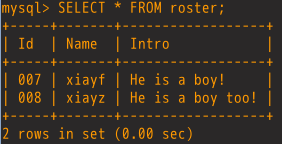
\includegraphics[height=2.5cm]{select.png}
	\end{figure}
	\end{center}
\end{frame}

\begin{frame}{删}
	\begin{block}{从表中删除一条记录}
	mysql$>${\bf DELETE FROM} roster {\bf WHERE} Name = "xiayz";\\
	Query OK, 1 row affected (0.00 sec)
	\end{block}
	\begin{block}{查询结果}
	mysql$>${\bf SELECT} * {\bf FROM} roster;\\
	{\color{blue}
	$+$-----$+$-------$+$---------------$+$\\
	$\mid$\ \ Id\ \ $\mid$\ Name\ $\mid$\ \ \ \ \ Intro\ \ \ \ \ $\mid$\\
	$+$-----$+$-------$+$---------------$+$\\
	$\mid$\ 007\ $\mid$\ \ xiayf\ $\mid$\ He is a boy!$\mid$\\
	$+$-----$+$-------$+$---------------$+$\\
	1 row in set (0.00 sec)}
	\end{block}
\end{frame}

\begin{frame}{改}
\begin{columns}
	\column[t]{5cm}
	{\small
	\begin{block}{查询表中所有记录}
	mysql$>${\bf SELECT} * {\bf FROM} roster;
	\end{block}
	\begin{block}{更改ID="009"的人员的Name}
	{\tiny
	mysql$>${\bf UPDATE} roster {\bf SET} Name="xiayongqing" {\bf WHERE} Id="009";\\
	{\color{blue}Query OK, 1 row affected (0.00 sec)\\
	Rows matched: 1 Changed: 1 Warning: 0}
	}
	\end{block}
	}
	\column[t]{5cm}
	\begin{flushright}
	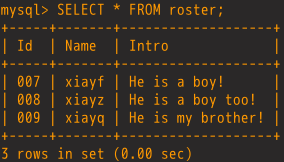
\includegraphics[width=4cm]{selectBeforeDelete.png}\\
	
	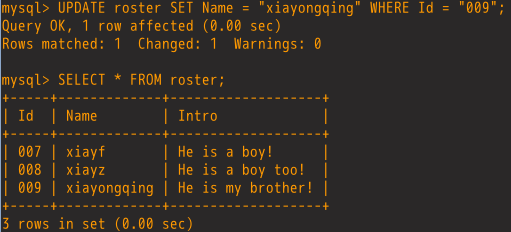
\includegraphics[width=6cm]{deleteAndSelect.png}
	\end{flushright}
\end{columns}
\end{frame}

\begin{frame}{查}
	\begin{itemize}
		\item SELECT Name FROM roster;
		\item SELECT Name FROM roster WHERE Id = "007";
		\item SELECT Id, Intro FROM roster WHERE Name = "xiayf";
		\item SELECT * FROM roster ORDER BY Name;
		\item SELECT Name, Intro FROM WHERE Name LIKE 'xia\%';\footnote{字符\%是代表任意字符串的通配符} 
	\end{itemize}
\end{frame}
\section{MySQL字符集问题}
\subsection{查看默认字符集}
\begin{frame}{默认字符集}
	\begin{block}{查看默认字符集}
	mysql$>$SHOW VARIABLES LIKE 'character\%';
	\end{block}
	\begin{block}{结果}
	\begin{tabular}{l|p{5cm}}\hline
	Variable\underline{\ }name & Value\\ \hline
	character\underline{\ }set\underline{\ }client & utf8\\
	character\underline{\ }set\underline{\ }connection & utf8\\
	character\underline{\ }set\underline{\ }database & utf8\\
	character\underline{\ }set\underline{\ }filesystem & binary\\
	character\underline{\ }set\underline{\ }results & utf8\\
	character\underline{\ }set\underline{\ }server & utf8\\
	character\underline{\ }set\underline{\ }system & utf8\\
	character\underline{\ }sets\underline{\ }dir & /usr/share/mysql/charsets/\\ \hline
	\end{tabular}
	\end{block}
\end{frame}
\subsection{修改默认字符集}
\begin{frame}{修改默认字符集}
	\begin{itemize}
		\item SET character\underline{\ }set\underline{\ }client = utf8;
		\item SET character\underline{\ }set\underline{\ }connection = utf8;
		\item ... 
	\end{itemize}
{\small 一般就算设置了表的默认字符集为utf8并且通过UTF-8编码发送查询,你会发现存入数据库的仍然是乱码。问题就出在这个connection连接层上。解决方法是在发送查询前执行下面这句:}
	\begin{block}{}
	SET NAMES 'utf8';	
	\end{block}
	它相当于下面的三句指令:
	\begin{block}{}
		\begin{itemize}
			\item SET character\underline{\ }set\underline{\ }client = utf8;
			\item SET character\underline{\ }set\underline{\ }results = utf8;
			\item SET character\underline{\ }set\underline{\ }connection = utf8;
		\end{itemize}
	\end{block}
\end{frame}
\begin{frame}
	\begin{center}
	{\LARGE THANK YOU !}
	\end{center}
	\begin{block}{}
	\begin{center}
	{\small Proud to use \LaTeX\ and Beamer.}
	\end{center}
	\end{block}
\end{frame}
\end{CJK*}
\end{document}
